\section{Radionuclide Transport Base Cases}\label{sec:nuclide_base_cases}
\subsection{Basic Transport and Containment Problem Specification}
The basic transport and containment base cases verify basic transport and 
contaminant behavior of all the radionuclide transport models at each component 
interface. These tests neglected thermal transport and capacity estimation to 
simplify the verification procedure. 

The problem design includes : 
\begin{itemize}
\item{A source facility providing one waste stream per timestep}
\item{A legislated repository capacity of 5 1kg waste streams}
\item{A waste form Component} 
\item{A waste package Component}
\item{A buffer Component}
\item{A far field Component}
\end{itemize}

\subsubsection{Degradation Rate Model}
The Degradation Rate model should not release contaminants if the degradation 
rate is 0. If the degradation rate is nonzero, however, contaminants should 
become available immediately to the adjacent components, traveling quickly 
accross the interfaces. 

To observe these behaviors, four simulations were run to demonstrate that total 
containment resulted from a degradation rate of 0 and that conrguent release 
resulted from nonzero degradation rates. A description of these verification 
cases can be found in Table \ref{tab:dr_no_release}. The 0 degradation rate component was 
different for each of the four cases. This resulted in total containment at the 
Waste Form, Waste Package, Buffer, and Far Field interfaces respectively. 
Results of these base cases can be found in Figures 
\ref{fig:drIwf5} through \ref{fig:drIVff0}.

\begin{table}
\centering
\footnotesize{
\begin{tabularx}{\textwidth}{|X|c|c|r|r|}
  \multicolumn{5}{c}{\textbf{Degradation Rate Model No Release Contaminant Transport}}\\
  \hline
  \textbf{Case}  &  \textbf{Component} &  \textbf{Degradation Rate} & \textbf{Expected 10 yrs} & \textbf{Actual 10 yrs}\\
  \textbf{ID}    & \textbf{[Type]} &  \textbf{$[yr^{-1}]$}  &  $[\%]$  & $[\%]$\\
  \hline
  DRI     &  WF    &  0   & 1 & 1\\
          &  WP    &  0.1 & 0 & 0 \\
          &  BUFF  &  0.1 & 0 & 0 \\
          &  FF    &  0.1 & 0 & 0\\
  \hline
  DRII    &  WF    &  0.1 & 0 & 0\\
          &  WP    &  0   & 1 & 1\\
          &  BUFF  &  0.1 & 0 & 0\\
          &  FF    &  0.1 & 0 & 0\\
  \hline
  DRIII   &  WF    &  0.1 & 0 & 0\\
          &  WP    &  0.1 & 0 & 0\\
          &  BUFF  &  0   & 1 & 1\\
          &  FF    &  0.1 & 0 & 0\\
  \hline
  DRIV    &  WF    &  0.1 & 0 & 0\\
          &  WP    &  0.1 & 0 & 0\\
          &  BUFF  &  0.1 & 0 & 0\\
          &  FF    &  0   & 1 & 1\\
  \hline
\end{tabularx}
\caption[Degradation rate model no release problem results.]{Results from demonstration cases for non-release from 0-degradation Degradation Rate modeled Components.}
\label{tab:dr_no_release}
}
\end{table}

\begin{figure}[ht]
\begin{minipage}[b]{0.45\linewidth}
\centering
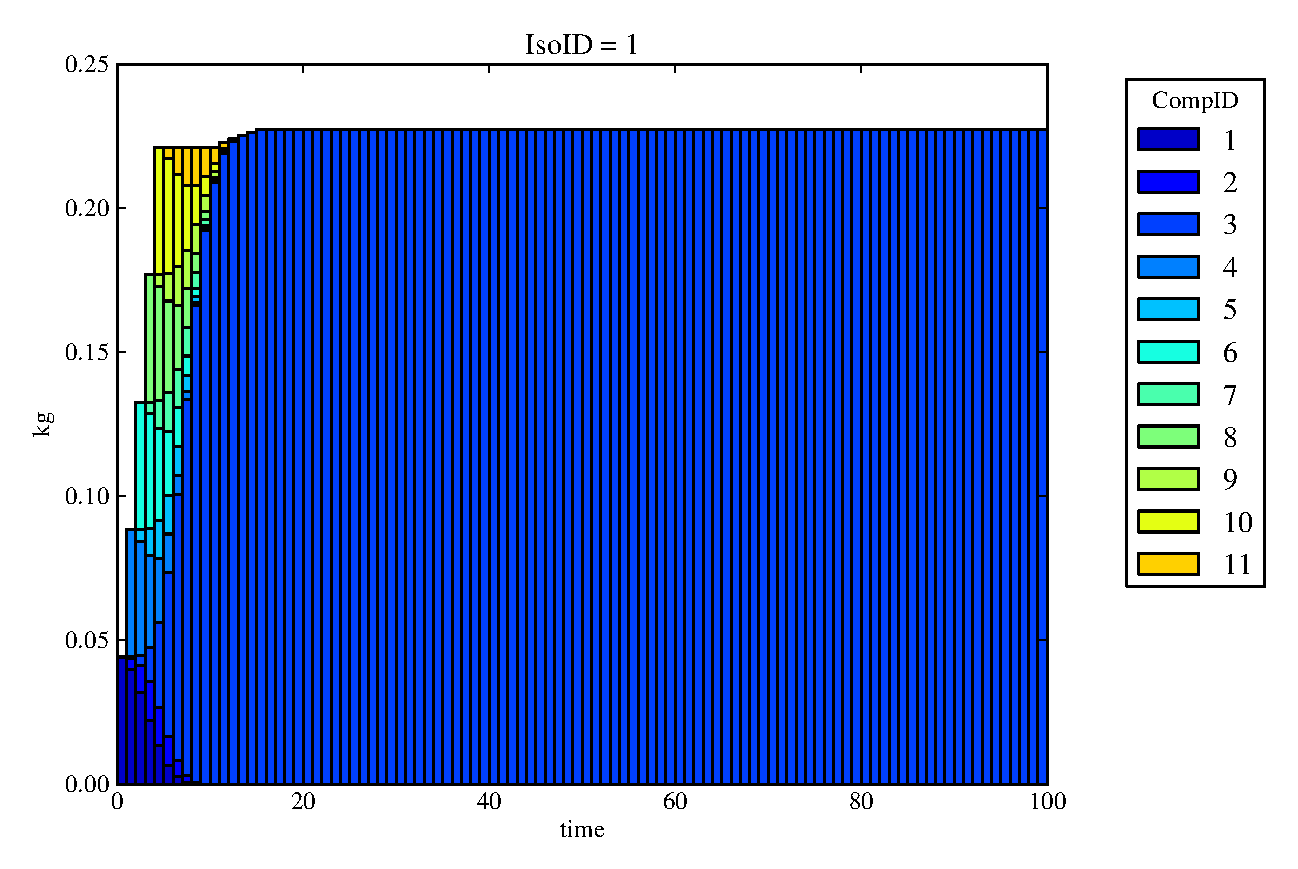
\includegraphics[width=\textwidth]{./chapters/demonstration/no_release/buff0deg.eps}
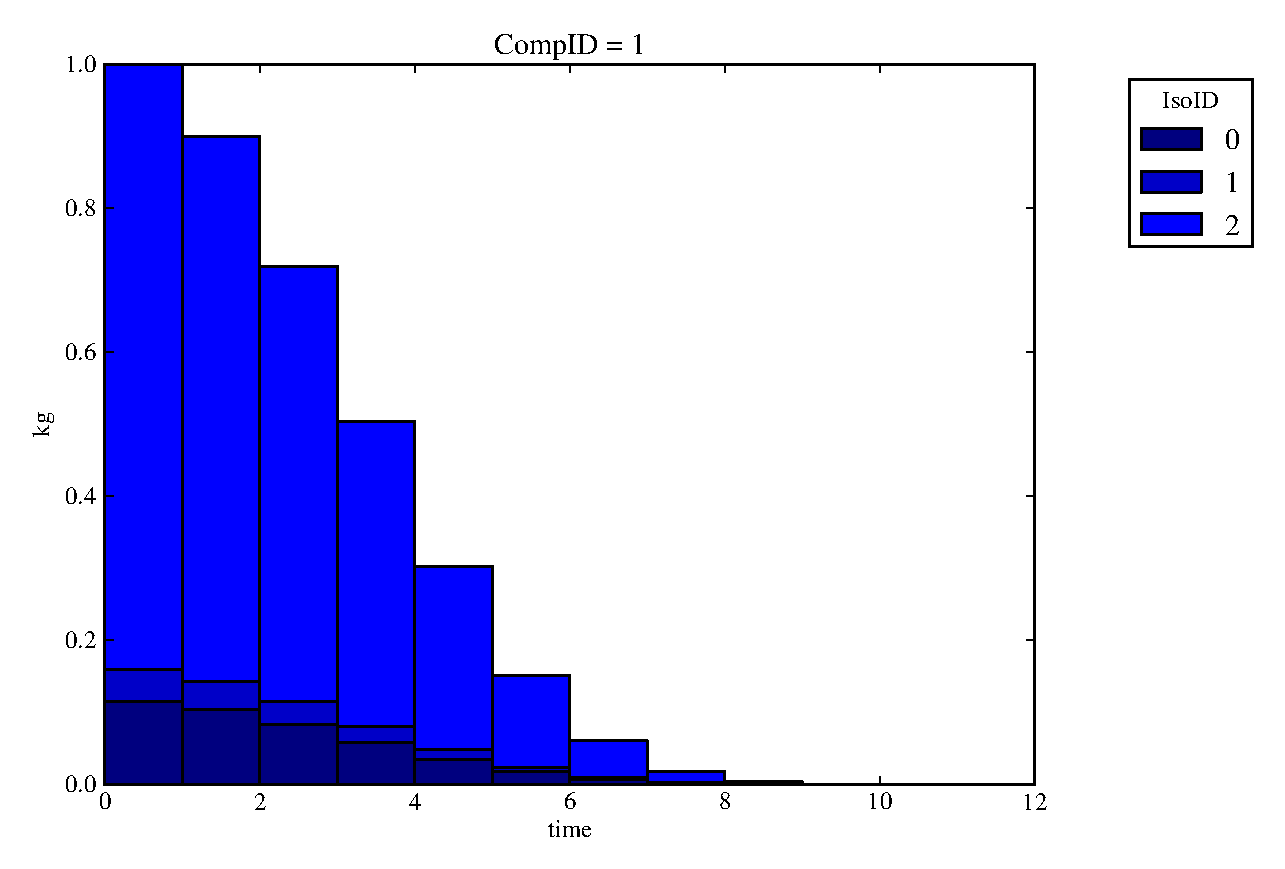
\includegraphics[width=\textwidth]{./chapters/demonstration/no_release/buff0deg1.eps}
\caption{default}
\label{fig:figure1}
\end{minipage}
\hspace{0.5cm}
\begin{minipage}[b]{0.45\linewidth}
\centering
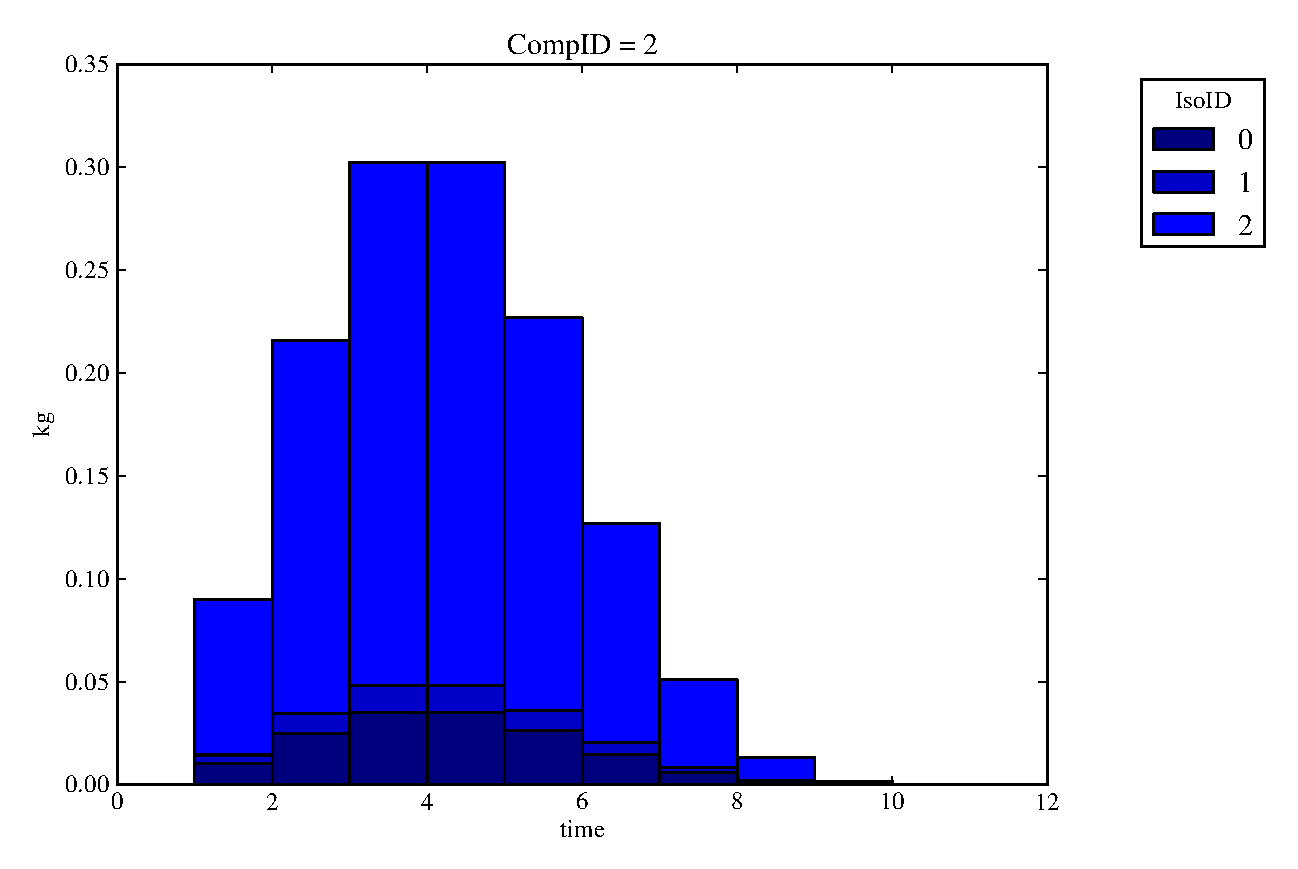
\includegraphics[width=\textwidth]{./chapters/demonstration/no_release/buff0deg2.eps}
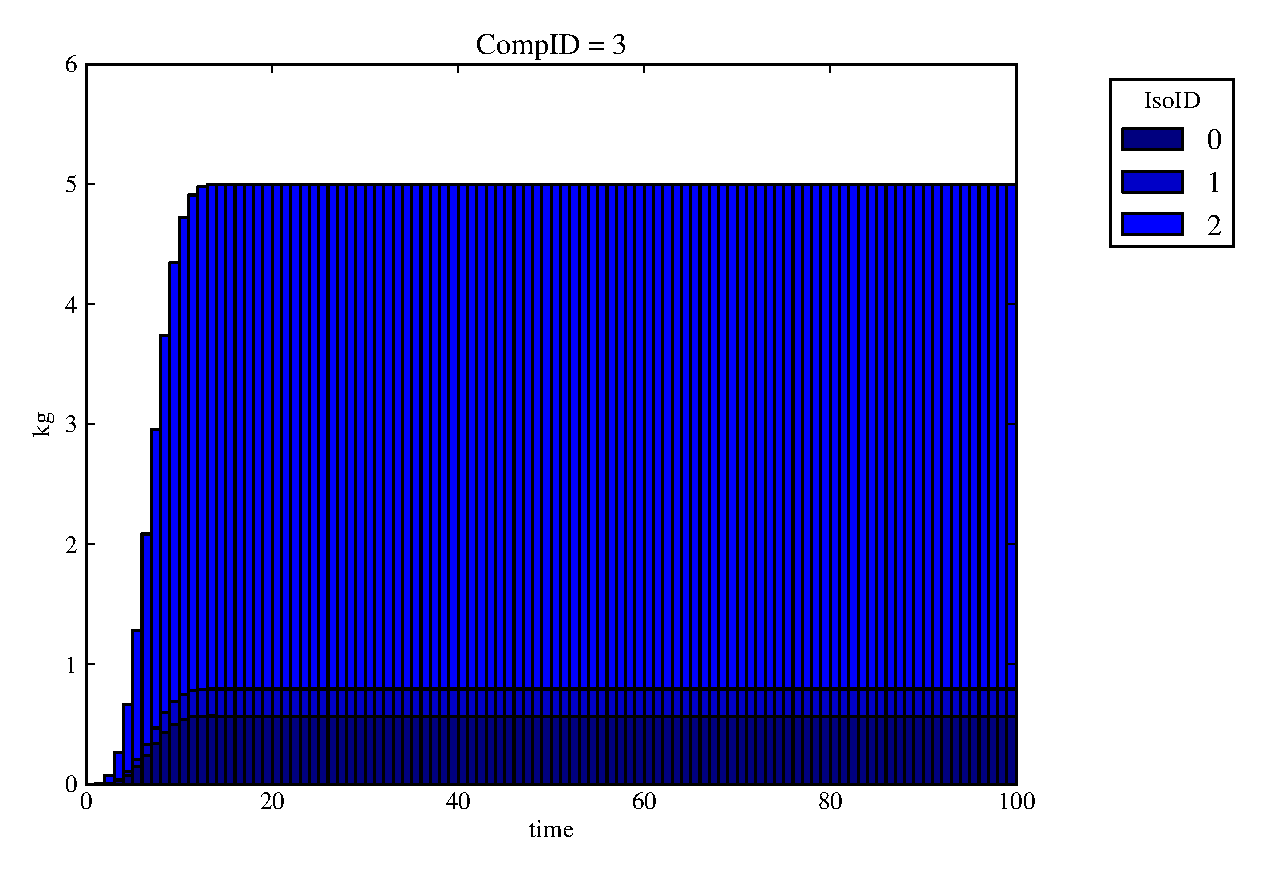
\includegraphics[width=\textwidth]{./chapters/demonstration/no_release/buff0deg3.eps}
\caption{default}
\label{fig:figure2}
\end{minipage}
\end{figure}

\clearpage

\subsubsection{Mixed Cell Model}
The Mixed Cell model behaves exactly similarly to the Degradation Rate 
model, when sorption and solubility limitation in that model are disabled. When they are 
enabled, however, expected to demonstrate sorption limited and solubility 
limited transport. The extent to which sorption and solubility limitation meet 
expectations is addressed in this base case.

Dual and single parameter verification cases were run to explore the effects of sorption and 
solubility limitation both separately and together. A description of these verification 
cases can be found in Table \ref{tab:mc_no_release}. 
Results of these base cases can be found in Figures \ref{fig:mcI} through 
\ref{fig:mcIV}.

\begin{table}
\centering
\begin{tabular}{|l|c|c|r|r|}
  \hline
  \multicolumn{5}{c}{\textbf{Mixed Cell Model No Release Contaminant Transport}}\\
  \hline
  \textbf{Case}  &  \textbf{Component} &  \textbf{Degradation Rate} & \textbf{Expected 10 yrs} & \textbf{Actual 10 yrs}\\
  \textbf{ID}    & \textbf{[Type]} &  \textbf{$[yr^{-1}]$}  &  $[\%]$  & $[\%]$\\
  \hline
  MCI     &  WF    &  0   & 1\\
          &  WP    &  0.1 & 0\\
          &  BUFF  &  0.1 & 0\\
          &  FF    &  0.1 & 0\\
  \hline
  MCII    &  WF    &  0.1 & 0\\
          &  WP    &  0   & 1\\
          &  BUFF  &  0.1 & 0\\
          &  FF    &  0.1 & 0\\
  \hline
  MCIII   &  WF    &  0.1 & 0\\
          &  WP    &  0.1 & 0\\
          &  BUFF  &  0   & 1\\
          &  FF    &  0.1 & 0\\
  \hline
  MCIV    &  WF    &  0.1 & 0\\
          &  WP    &  0.1 & 0\\
          &  BUFF  &  0.1 & 0\\
          &  FF    &  0   & 1\\
  \hline
\end{tabular}
\caption{<+Caption text+>}
\label{tab:<+label+>}
\end{table}<++>

\begin{figure}[ht]
\centering
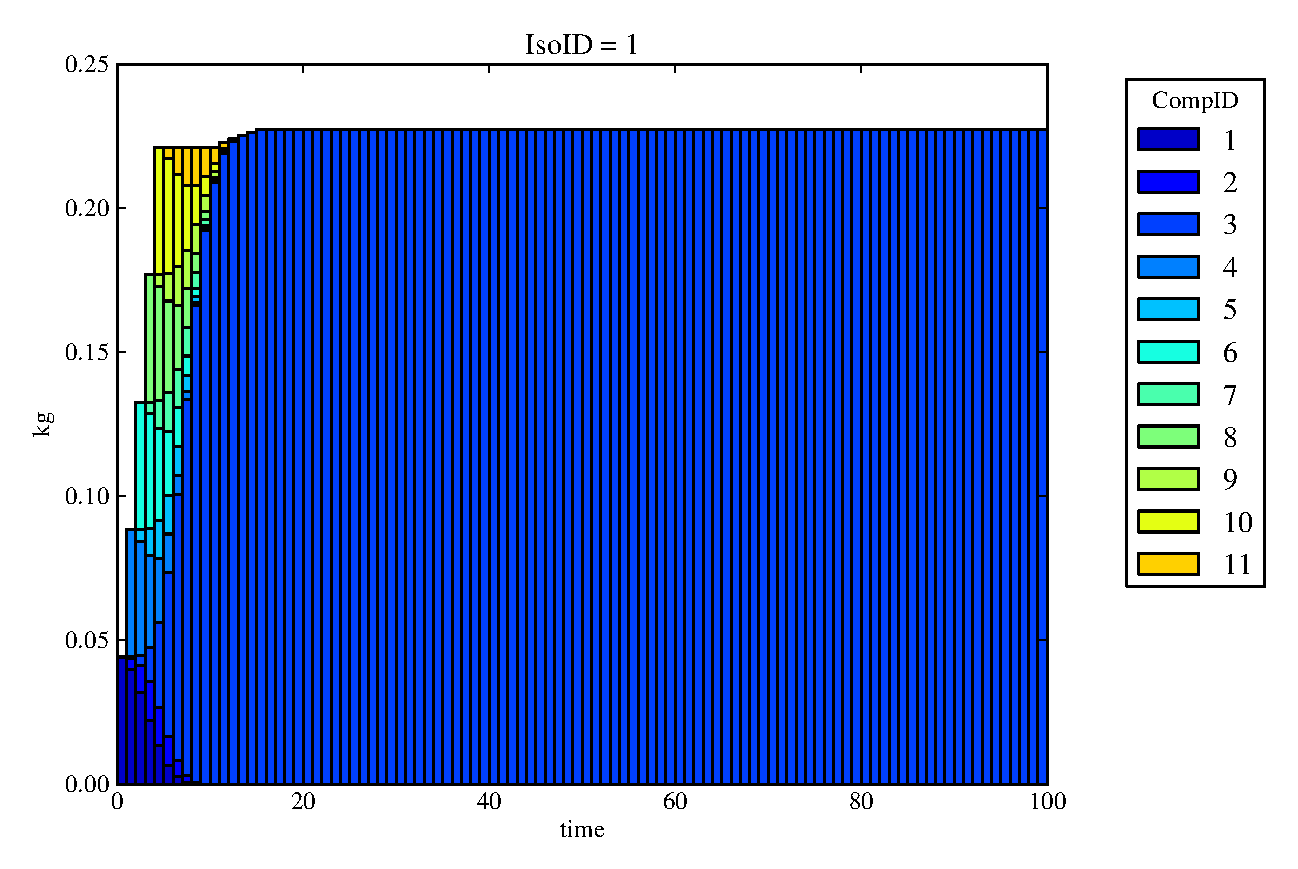
\includegraphics[width=0.8\textwidth]{./chapters/demonstration/no_release/buff0deg.eps}
\caption[$^{235}U$ residence. Degradation Rate <+Component+> No Release.]{
For <+CASE+> case in which total containment in the <+component+> is assumed 
($F_{d,<+comp+>}=0$), $^{235}U$ travels through <++> components ($F_d = 0.1$) before 
permanent residence in the <+component+> component.
}
\label{fig:drIIIall}
\begin{minipage}[b]{0.45\linewidth}

  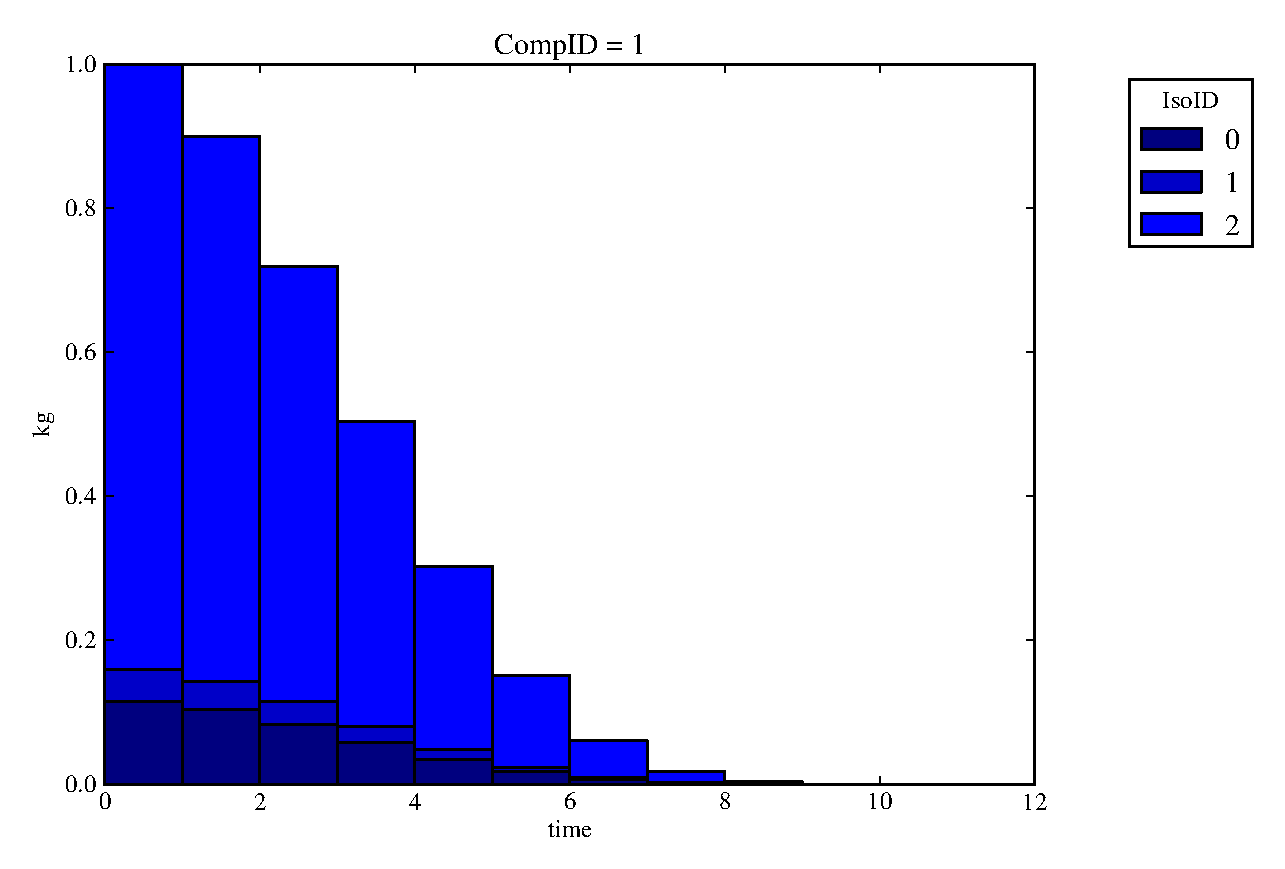
\includegraphics[width=\textwidth]{./chapters/demonstration/no_release/buff0deg1.eps}
  \caption[DRIII Waste Form Contaminants.]{
    Waste Form 5 ($F_d = 0.1$) releases material with degradation. 
    }
  \label{fig:drIIIwf5}
  
  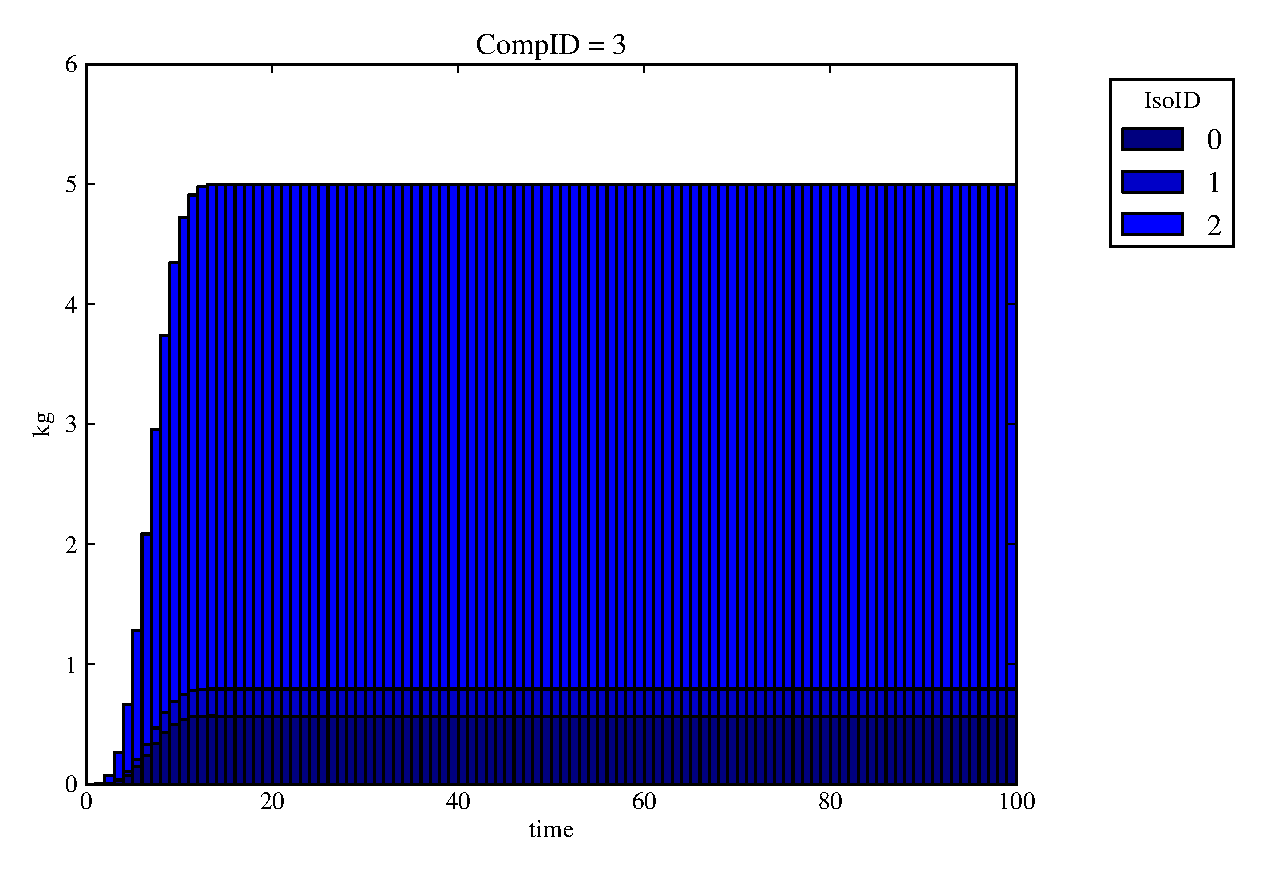
\includegraphics[width=\textwidth]{./chapters/demonstration/no_release/buff0deg3.eps}
  \caption[Case DRIII Buffer Contaminants]{
    The Buffer, component 7 ($F_d=0$), acheives total containment.
    }
  \label{fig:drIIIbuff}

\end{minipage}
\hspace{0.05\linewidth}
\begin{minipage}[b]{0.45\linewidth}
  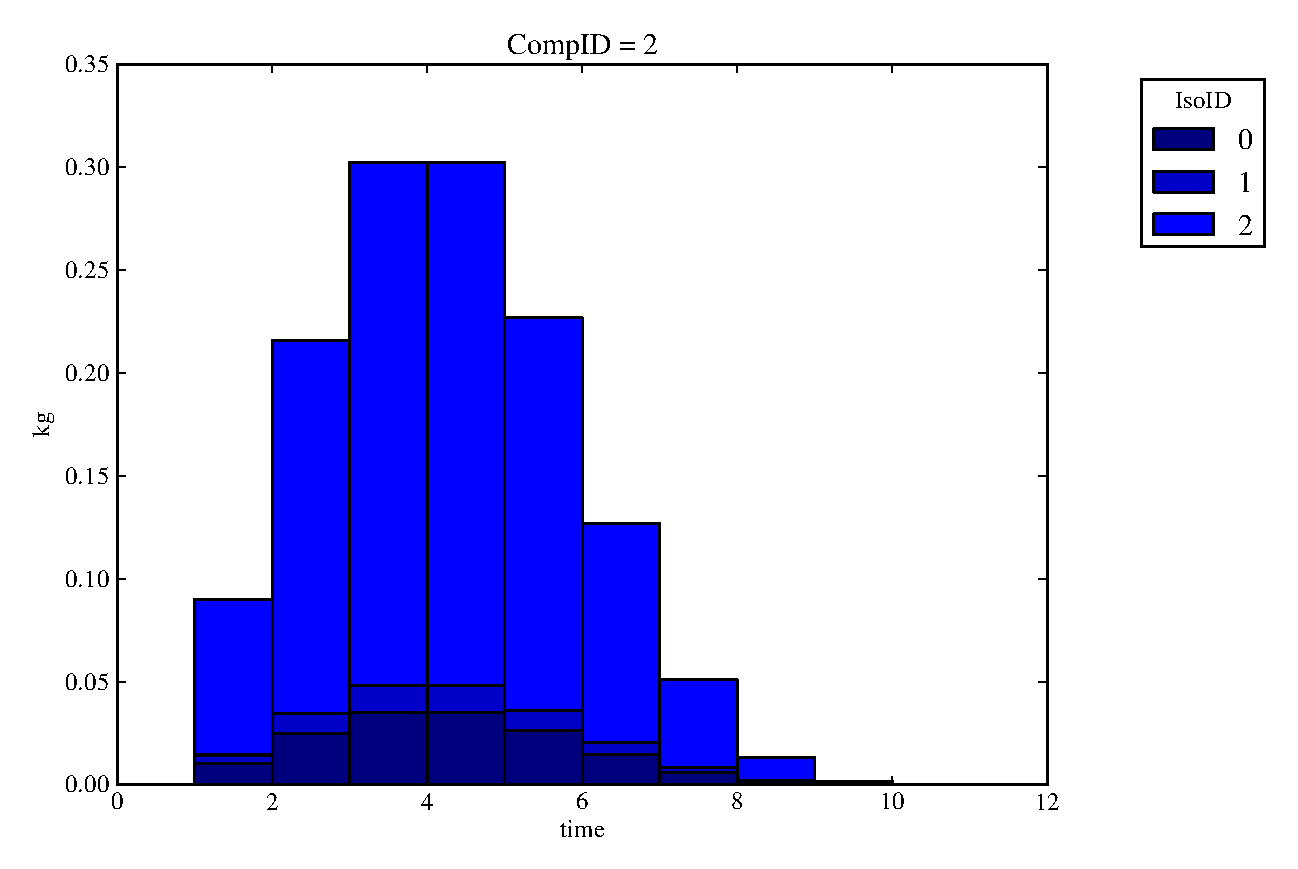
\includegraphics[width=\textwidth]{./chapters/demonstration/no_release/buff0deg2.eps}
  \caption[Case DRIII Waste Package Contaminants.]{ 
    Waste Package 6 ($F_d = 0.1$) recieves then releases material. 
    }
  \label{fig:drIIIwp6}

  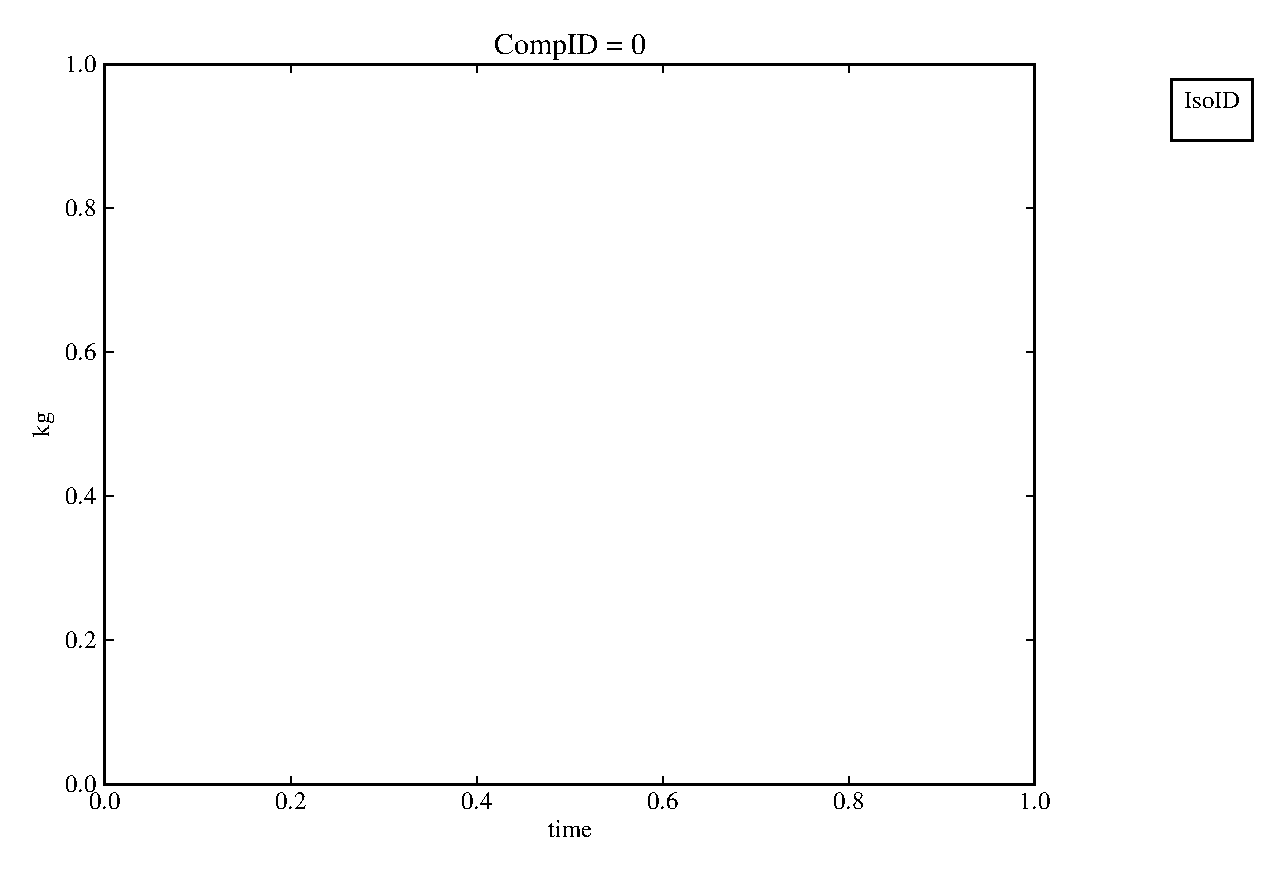
\includegraphics[width=\textwidth]{./chapters/demonstration/no_release/buff0deg0.eps}
  \caption[Case DRIII Waste Package Contaminants.]{ 
    The Far Field, component 0 ($F_d = 0.1$), never recieves material.
    }
  \label{fig:drIIIff0}


  \end{minipage}
\end{figure}

\clearpage

\subsubsection{Lumped Parameter Model}
The Lumped Parameter model, with its three formulations (Exponential Model, 
Dispersion Model, and Piston flow Model) is not expected to receive 
contaminants if the porosity or advective velocity are zero. Else, however, 
contaminants are expected to  become available to the adjacent components 
according to the functional forms of the formulations. 

To observe the behaviors of each of the three formulations and to demonstrate 
full containment in cases where it is expected, simulations were run
according to the descriptions in Table \ref{tab:lp_no_release}.
Results of these base cases can be found in Figures 
\ref{fig:lpEMI} through \ref{fig:lpPFMIV}.

\begin{table}
\centering
\begin{tabular}{|l|c|c|r|}
  \hline
  \multicolumn{4}{c}{\textbf{Lumped Parameter Model No Release Contaminant Transport}}\\
  \hline
  \textbf{Case}  &  \textbf{Component} &  \textbf{PFM Param} & \textbf{Expected 10 yrs} & \textbf{Actual 10 yrs}\\
  \textbf{ID}    & \textbf{[Type]} &  \textbf{$[yr^{-1}]$}  &  $[\%]$  & $[\%]$\\
  \hline
  DRI     &  WF    &  0   & 1\\
          &  WP    &  0.1 & 0\\
          &  BUFF  &  0.1 & 0\\
          &  FF    &  0.1 & 0\\
  \hline
  DRII    &  WF    &  0.1 & 0\\
          &  WP    &  0   & 1\\
          &  BUFF  &  0.1 & 0\\
          &  FF    &  0.1 & 0\\
  \hline
  DRIII   &  WF    &  0.1 & 0\\
          &  WP    &  0.1 & 0\\
          &  BUFF  &  0   & 1\\
          &  FF    &  0.1 & 0\\
  \hline
  DRIV    &  WF    &  0.1 & 0\\
          &  WP    &  0.1 & 0\\
          &  BUFF  &  0.1 & 0\\
          &  FF    &  0   & 1\\
  \hline
\end{tabular}
\caption{<+Caption text+>}
\label{tab:<+label+>}
\end{table}<++>

\begin{figure}[ht]
\centering
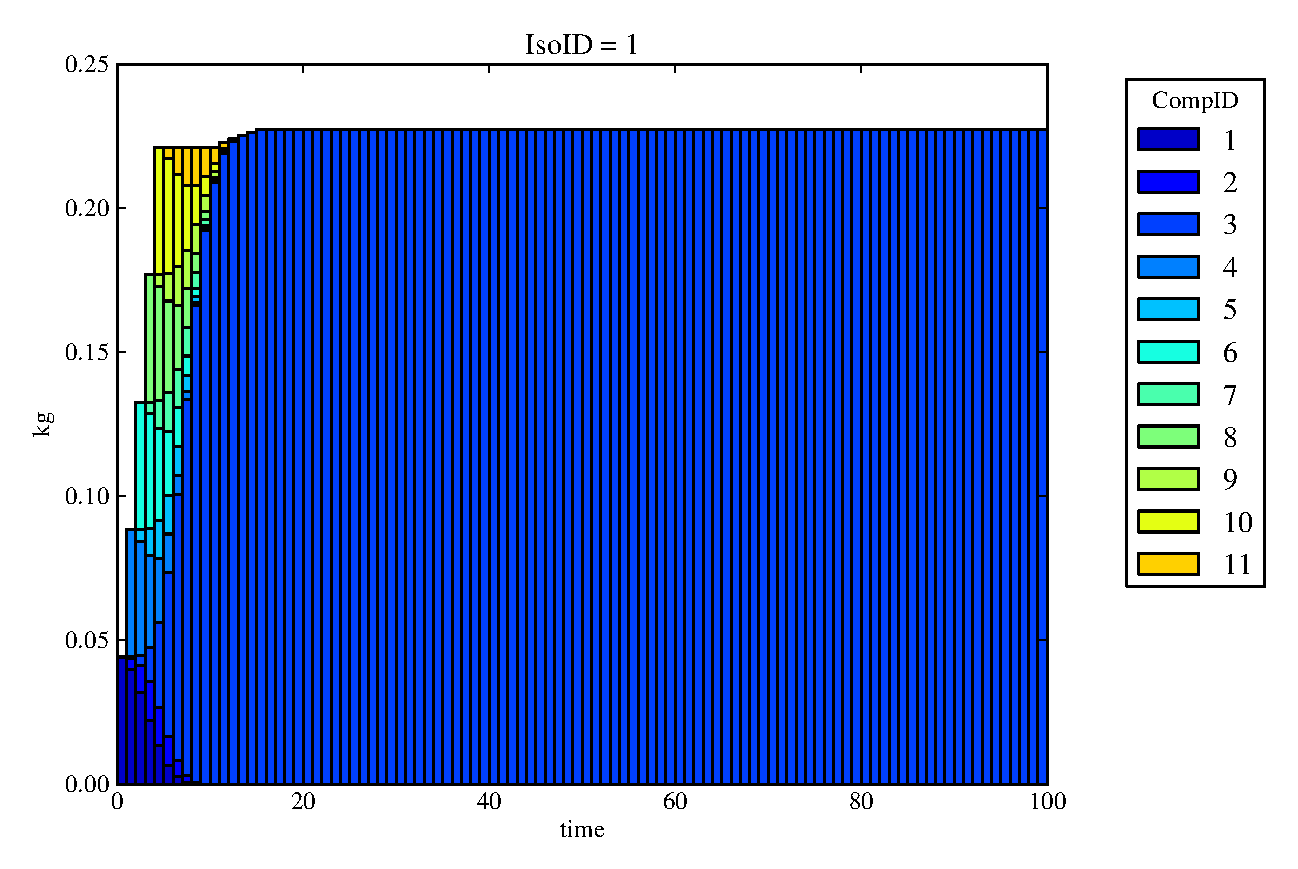
\includegraphics[width=0.8\textwidth]{./chapters/demonstration/no_release/buff0deg.eps}
\caption[$^{235}U$ residence. Degradation Rate <+Component+> No Release.]{
For <+CASE+> case in which total containment in the <+component+> is assumed 
($F_{d,<+comp+>}=0$), $^{235}U$ travels through <++> components ($F_d = 0.1$) before 
permanent residence in the <+component+> component.
}
\label{fig:drIIIall}
\begin{minipage}[b]{0.45\linewidth}

  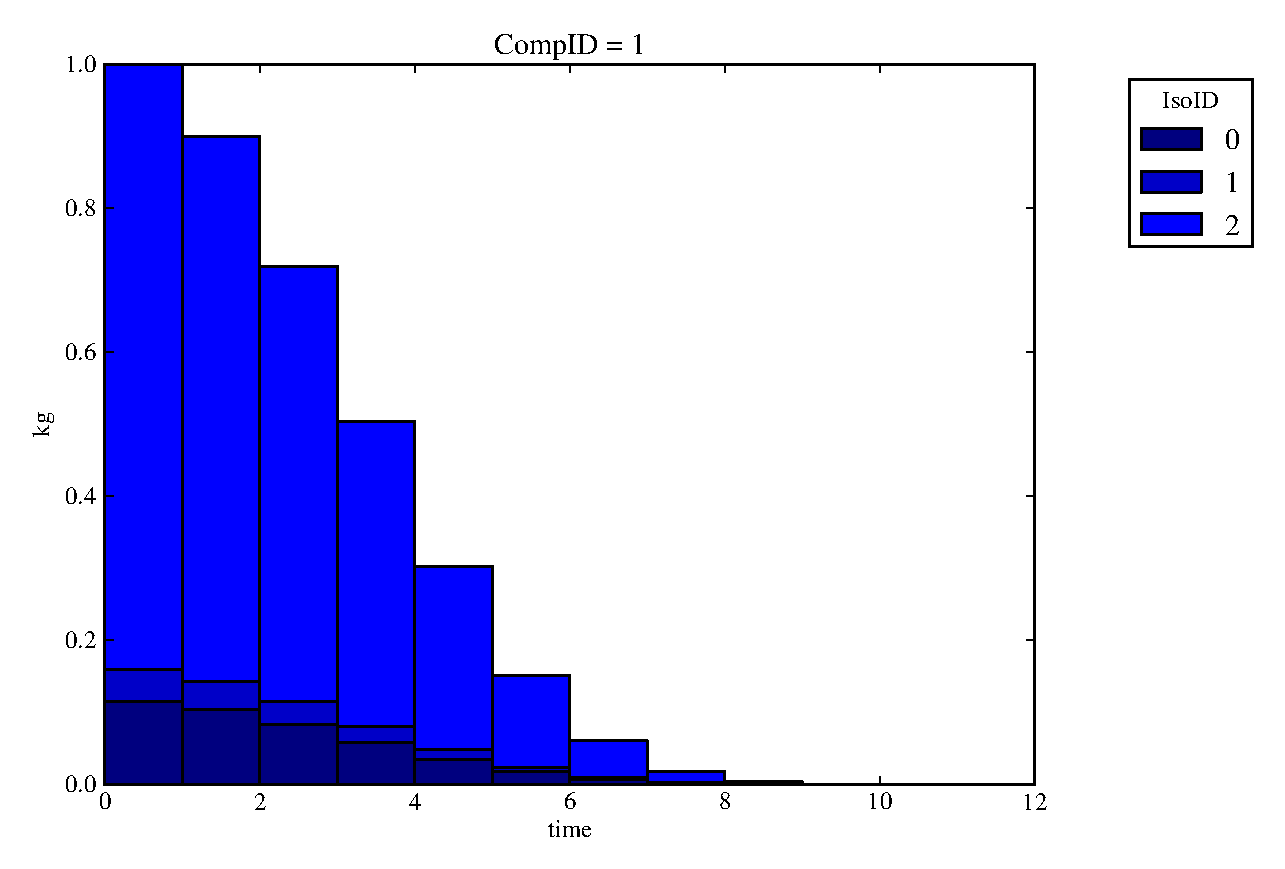
\includegraphics[width=\textwidth]{./chapters/demonstration/no_release/buff0deg1.eps}
  \caption[DRIII Waste Form Contaminants.]{
    Waste Form 5 ($F_d = 0.1$) releases material with degradation. 
    }
  \label{fig:drIIIwf5}
  
  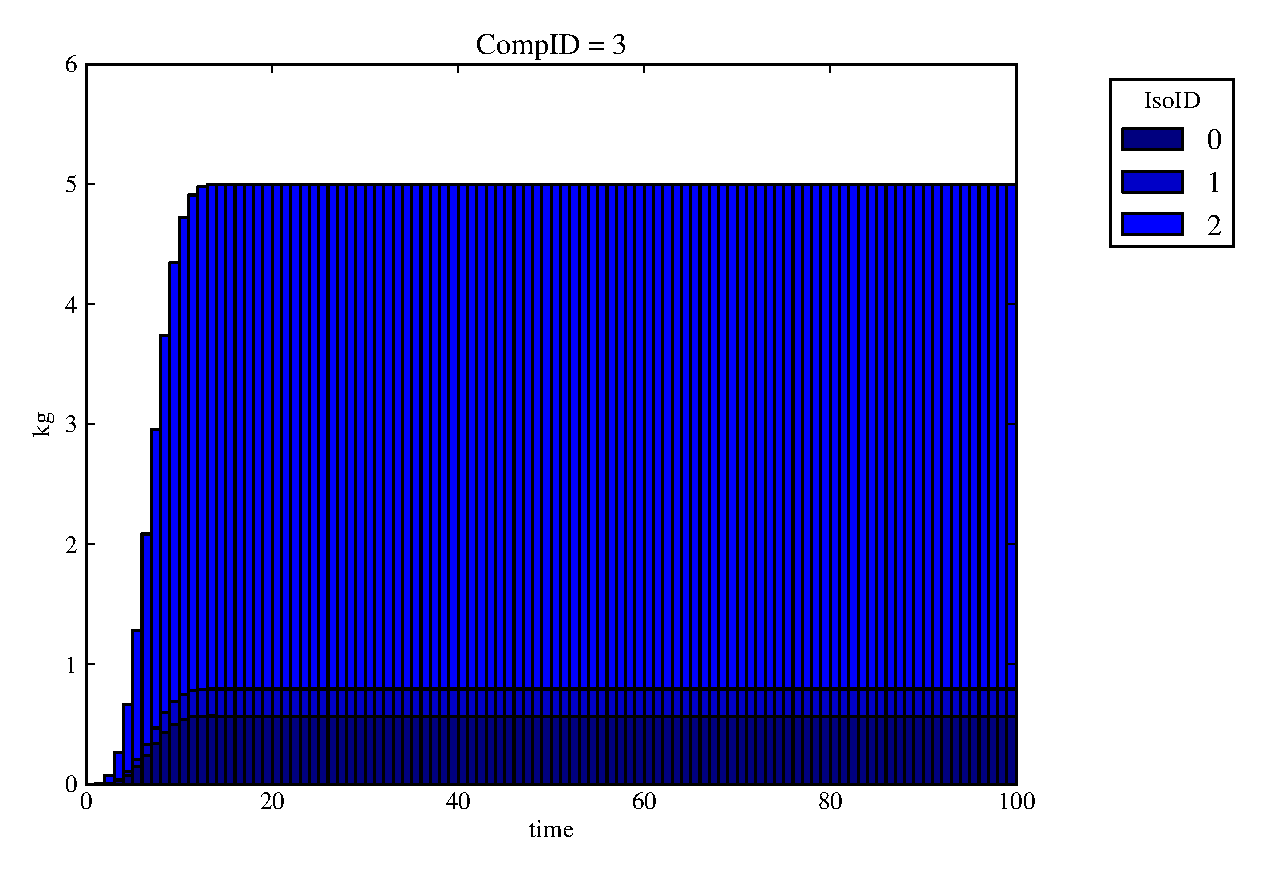
\includegraphics[width=\textwidth]{./chapters/demonstration/no_release/buff0deg3.eps}
  \caption[Case DRIII Buffer Contaminants]{
    The Buffer, component 7 ($F_d=0$), acheives total containment.
    }
  \label{fig:drIIIbuff}

\end{minipage}
\hspace{0.05\linewidth}
\begin{minipage}[b]{0.45\linewidth}
  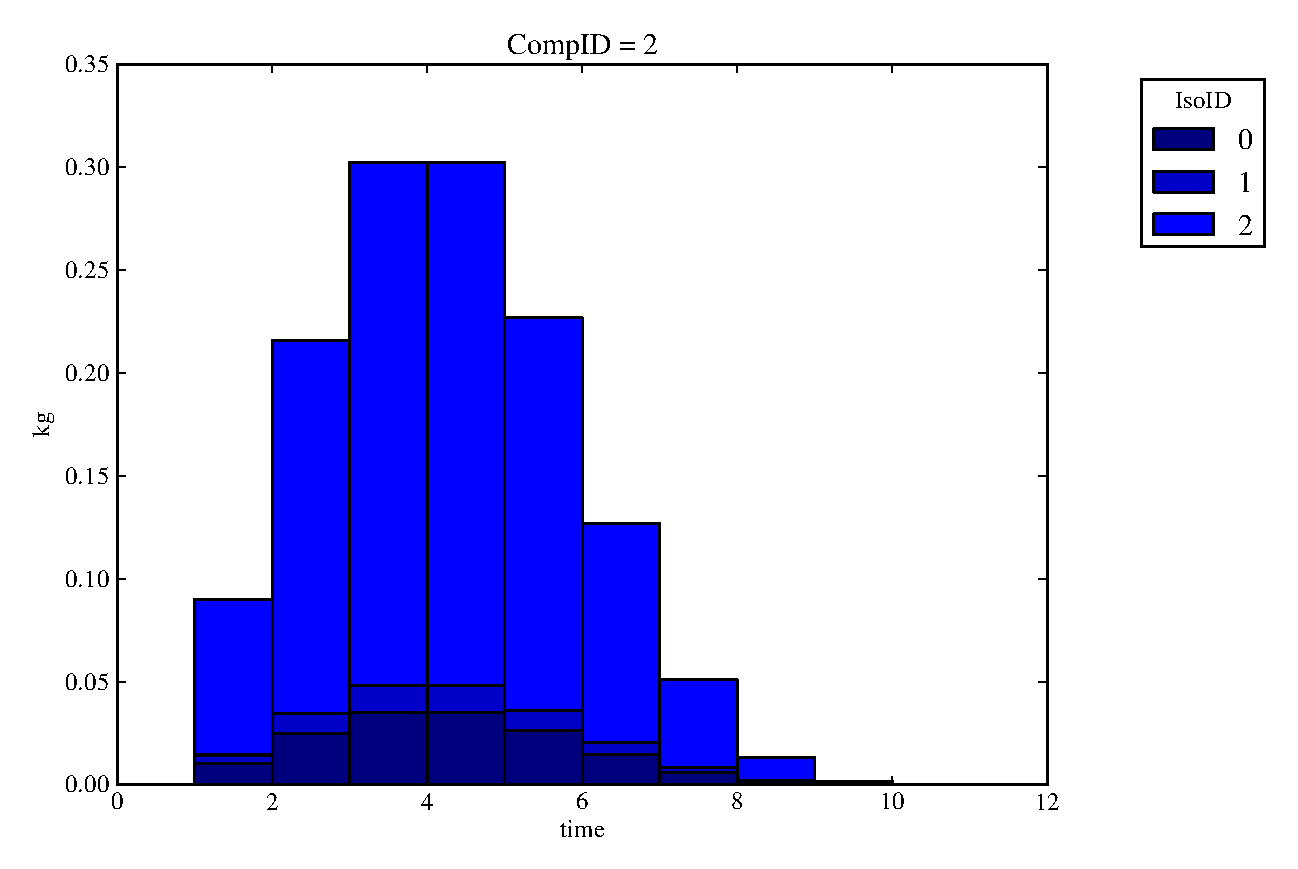
\includegraphics[width=\textwidth]{./chapters/demonstration/no_release/buff0deg2.eps}
  \caption[Case DRIII Waste Package Contaminants.]{ 
    Waste Package 6 ($F_d = 0.1$) recieves then releases material. 
    }
  \label{fig:drIIIwp6}

  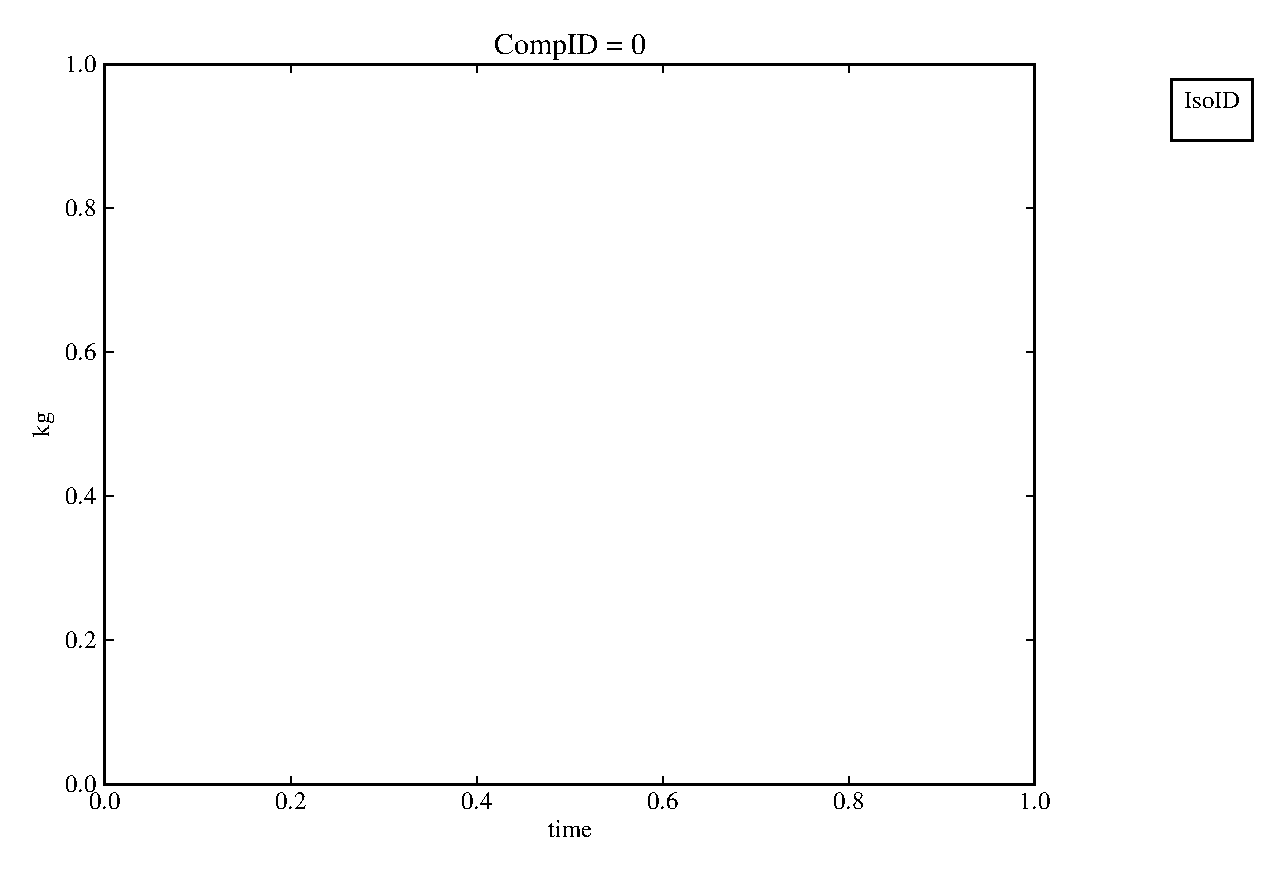
\includegraphics[width=\textwidth]{./chapters/demonstration/no_release/buff0deg0.eps}
  \caption[Case DRIII Waste Package Contaminants.]{ 
    The Far Field, component 0 ($F_d = 0.1$), never recieves material.
    }
  \label{fig:drIIIff0}


  \end{minipage}
\end{figure}

\clearpage

\subsubsection{One Dimensional Advecitive Dispersive Model}
The One Dimensional Advective Dispersive Model contaminants if the porosity is 
zero or if both the reference diffusivity and advective velocity are zero. 
Else, however, contaminants are expected to  become available to the adjacent 
components according to the analytical form of the solution.

To observe the behavior of the solution and to demonstrate full containment in 
cases where it is expected, simulations were run according to the descriptions 
in Table \ref{tab:1d_no_release}.  Results of these base cases can be found in 
Figures \ref{fig:1dI} through \ref{fig:1dIV}.  

\begin{table}
\centering
\begin{tabular}{|l|c|c|r|r|}
  \hline
  \multicolumn{5}{c}{\textbf{One Dimensional PPM Model No Release Contaminant Transport}}\\
  \hline
  \textbf{Case}  &  \textbf{Component} &  \textbf{Porosity} & \textbf{Expected 10 yrs} & \textbf{Actual 10 yrs}\\
  \textbf{ID}    & \textbf{[Type]} &  \textbf{$[yr^{-1}]$}  &  $[\%]$  & $[\%]$\\
  \hline
  DRI     &  WF    &  0   & 1\\
          &  WP    &  0.1 & 0\\
          &  BUFF  &  0.1 & 0\\
          &  FF    &  0.1 & 0\\
  \hline
  DRII    &  WF    &  0.1 & 0\\
          &  WP    &  0   & 1\\
          &  BUFF  &  0.1 & 0\\
          &  FF    &  0.1 & 0\\
  \hline
  DRIII   &  WF    &  0.1 & 0\\
          &  WP    &  0.1 & 0\\
          &  BUFF  &  0   & 1\\
          &  FF    &  0.1 & 0\\
  \hline
  DRIV    &  WF    &  0.1 & 0\\
          &  WP    &  0.1 & 0\\
          &  BUFF  &  0.1 & 0\\
          &  FF    &  0   & 1\\
  \hline
\end{tabular}
\caption{<+Caption text+>}
\label{tab:<+label+>}
\end{table}<++>


\begin{figure}[ht]
\centering
\includegraphics[width=0.8\textwidth]{./chapters/demonstration/no_release/lpI.eps}
\caption[$^{235}U$ residence. Lumped Parameter  <+Component+> No Release.]{
For <+CASE+> case in which total containment in the <+component+> is assumed 
($F_{d,<+comp+>}=0$), $^{235}U$ travels through <++> components ($F_d = 0.1$) before 
permanent residence in the <+component+> component.
}
\label{fig:lpIall}
\begin{minipage}[b]{0.45\linewidth}

  \includegraphics[width=\textwidth]{./chapters/demonstration/no_release/lpI1.eps}
  \caption[1DI Waste Form Contaminants.]{
    Waste Form 5 ($F_d = 0.1$) releases material with degradation. 
    }
  \label{fig:lpIwf5}
  
  \includegraphics[width=\textwidth]{./chapters/demonstration/no_release/lpI3.eps}
  \caption[Case 1DI Buffer Contaminants]{
    The Buffer, component 7 ($F_d=0$), acheives total containment.
    }
  \label{fig:lpIbuff}

\end{minipage}
\hspace{0.05\linewidth}
\begin{minipage}[b]{0.45\linewidth}
  \includegraphics[width=\textwidth]{./chapters/demonstration/no_release/lpI2.eps}
  \caption[Case 1DI Waste Package Contaminants.]{ 
    Waste Package 6 ($F_d = 0.1$) recieves then releases material. 
    }
  \label{fig:lpIwp6}

  \includegraphics[width=\textwidth]{./chapters/demonstration/no_release/lpI0.eps}
  \caption[Case 1DI Waste Package Contaminants.]{ 
    The Far Field, component 0 ($F_d = 0.1$), never recieves material.
    }
  \label{fig:lpIff0}


  \end{minipage}
\end{figure}
\begin{figure}[ht]
\centering
\includegraphics[width=0.8\textwidth]{./chapters/demonstration/no_release/lpII.eps}
\caption[$^{235}U$ residence. Lumped Parameter  <+Component+> No Release.]{
For <+CASE+> case in which total containment in the <+component+> is assumed 
($F_{d,<+comp+>}=0$), $^{235}U$ travels through <++> components ($F_d = 0.1$) before 
permanent residence in the <+component+> component.
}
\label{fig:lpIIall}
\begin{minipage}[b]{0.45\linewidth}

  \includegraphics[width=\textwidth]{./chapters/demonstration/no_release/lpII1.eps}
  \caption[1DII Waste Form Contaminants.]{
    Waste Form 5 ($F_d = 0.1$) releases material with degradation. 
    }
  \label{fig:lpIIwf5}
  
  \includegraphics[width=\textwidth]{./chapters/demonstration/no_release/lpII3.eps}
  \caption[Case 1DII Buffer Contaminants]{
    The Buffer, component 7 ($F_d=0$), acheives total containment.
    }
  \label{fig:lpIIbuff}

\end{minipage}
\hspace{0.05\linewidth}
\begin{minipage}[b]{0.45\linewidth}
  \includegraphics[width=\textwidth]{./chapters/demonstration/no_release/lpII2.eps}
  \caption[Case 1DII Waste Package Contaminants.]{ 
    Waste Package 6 ($F_d = 0.1$) recieves then releases material. 
    }
  \label{fig:lpIIwp6}

  \includegraphics[width=\textwidth]{./chapters/demonstration/no_release/lpII0.eps}
  \caption[Case 1DII Waste Package Contaminants.]{ 
    The Far Field, component 0 ($F_d = 0.1$), never recieves material.
    }
  \label{fig:lpIIff0}


  \end{minipage}
\end{figure}
\begin{figure}[ht]
\centering
\includegraphics[width=0.8\textwidth]{./chapters/demonstration/no_release/lpIII.eps}
\caption[$^{235}U$ residence. Lumped Parameter  <+Component+> No Release.]{
For <+CASE+> case in which total containment in the <+component+> is assumed 
($F_{d,<+comp+>}=0$), $^{235}U$ travels through <++> components ($F_d = 0.1$) before 
permanent residence in the <+component+> component.
}
\label{fig:lpIIIall}
\begin{minipage}[b]{0.45\linewidth}

  \includegraphics[width=\textwidth]{./chapters/demonstration/no_release/lpIII1.eps}
  \caption[1DIII Waste Form Contaminants.]{
    Waste Form 5 ($F_d = 0.1$) releases material with degradation. 
    }
  \label{fig:lpIIIwf5}
  
  \includegraphics[width=\textwidth]{./chapters/demonstration/no_release/lpIII3.eps}
  \caption[Case 1DIII Buffer Contaminants]{
    The Buffer, component 7 ($F_d=0$), acheives total containment.
    }
  \label{fig:lpIIIbuff}

\end{minipage}
\hspace{0.05\linewidth}
\begin{minipage}[b]{0.45\linewidth}
  \includegraphics[width=\textwidth]{./chapters/demonstration/no_release/lpIII2.eps}
  \caption[Case 1DIII Waste Package Contaminants.]{ 
    Waste Package 6 ($F_d = 0.1$) recieves then releases material. 
    }
  \label{fig:lpIIIwp6}

  \includegraphics[width=\textwidth]{./chapters/demonstration/no_release/lpIII0.eps}
  \caption[Case 1DIII Waste Package Contaminants.]{ 
    The Far Field, component 0 ($F_d = 0.1$), never recieves material.
    }
  \label{fig:lpIIIff0}


  \end{minipage}
\end{figure}


\begin{figure}[ht]
\centering
\includegraphics[width=0.8\textwidth]{./chapters/demonstration/no_release/lpIV.eps}
\caption[$^{235}U$ residence. Lumped Parameter  <+Component+> No Release.]{
For <+CASE+> case in which total containment in the <+component+> is assumed 
($F_{d,<+comp+>}=0$), $^{235}U$ travels through <++> components ($F_d = 0.1$) before 
permanent residence in the <+component+> component.
}
\label{fig:lpIVall}
\begin{minipage}[b]{0.45\linewidth}

  \includegraphics[width=\textwidth]{./chapters/demonstration/no_release/lpIV1.eps}
  \caption[1DIV Waste Form Contaminants.]{
    Waste Form 5 ($F_d = 0.1$) releases material with degradation. 
    }
  \label{fig:lpIVwf5}
  
  \includegraphics[width=\textwidth]{./chapters/demonstration/no_release/lpIV3.eps}
  \caption[Case 1DIV Buffer Contaminants]{
    The Buffer, component 7 ($F_d=0$), acheives total containment.
    }
  \label{fig:lpIVbuff}

\end{minipage}
\hspace{0.05\linewidth}
\begin{minipage}[b]{0.45\linewidth}
  \includegraphics[width=\textwidth]{./chapters/demonstration/no_release/lpIV2.eps}
  \caption[Case 1DIV Waste Package Contaminants.]{ 
    Waste Package 6 ($F_d = 0.1$) recieves then releases material. 
    }
  \label{fig:lpIVwp6}

  \includegraphics[width=\textwidth]{./chapters/demonstration/no_release/lpIV0.eps}
  \caption[Case 1DIV Waste Package Contaminants.]{ 
    The Far Field, component 0 ($F_d = 0.1$), never recieves material.
    }
  \label{fig:lpIVff0}


  \end{minipage}
\end{figure}

\clearpage
